\section{Delaunay triangulation and voronoi tessellation}
A common method for examining the ordering and periodicity of large-scale crystalline structures is to generate a mesh with each vertex being the location of a particle. With this, we can easily observe ordered and disordered regions in a material; well defined straight lines indicate a perfect crystal, with any bends indicating the presence of imperfections. Some of the most widely used methods for this are the dual techniques from computational geometry of Delaunay triangulation, and voronoi tessellation.

The Delaunay triangulation of an arbitrary set of points in Euclidian space, $\mathbf{R}$, which I will denote as $D(\mathbf{R})$, is contructed between points by following:
\begin{enumerate}
    \item No point will fall within the interior of any circumcircle of 3 points where $\mathbf{r}_{1..3} \subset \mathbf{R}$
    \item The Delaunay triangulation will maximise the minimum angle between points.
    \item If four points are on the same circumcircle, then both possible configurations give a Delaunay triangulation.
\end{enumerate}

\begin{figure}\centering
    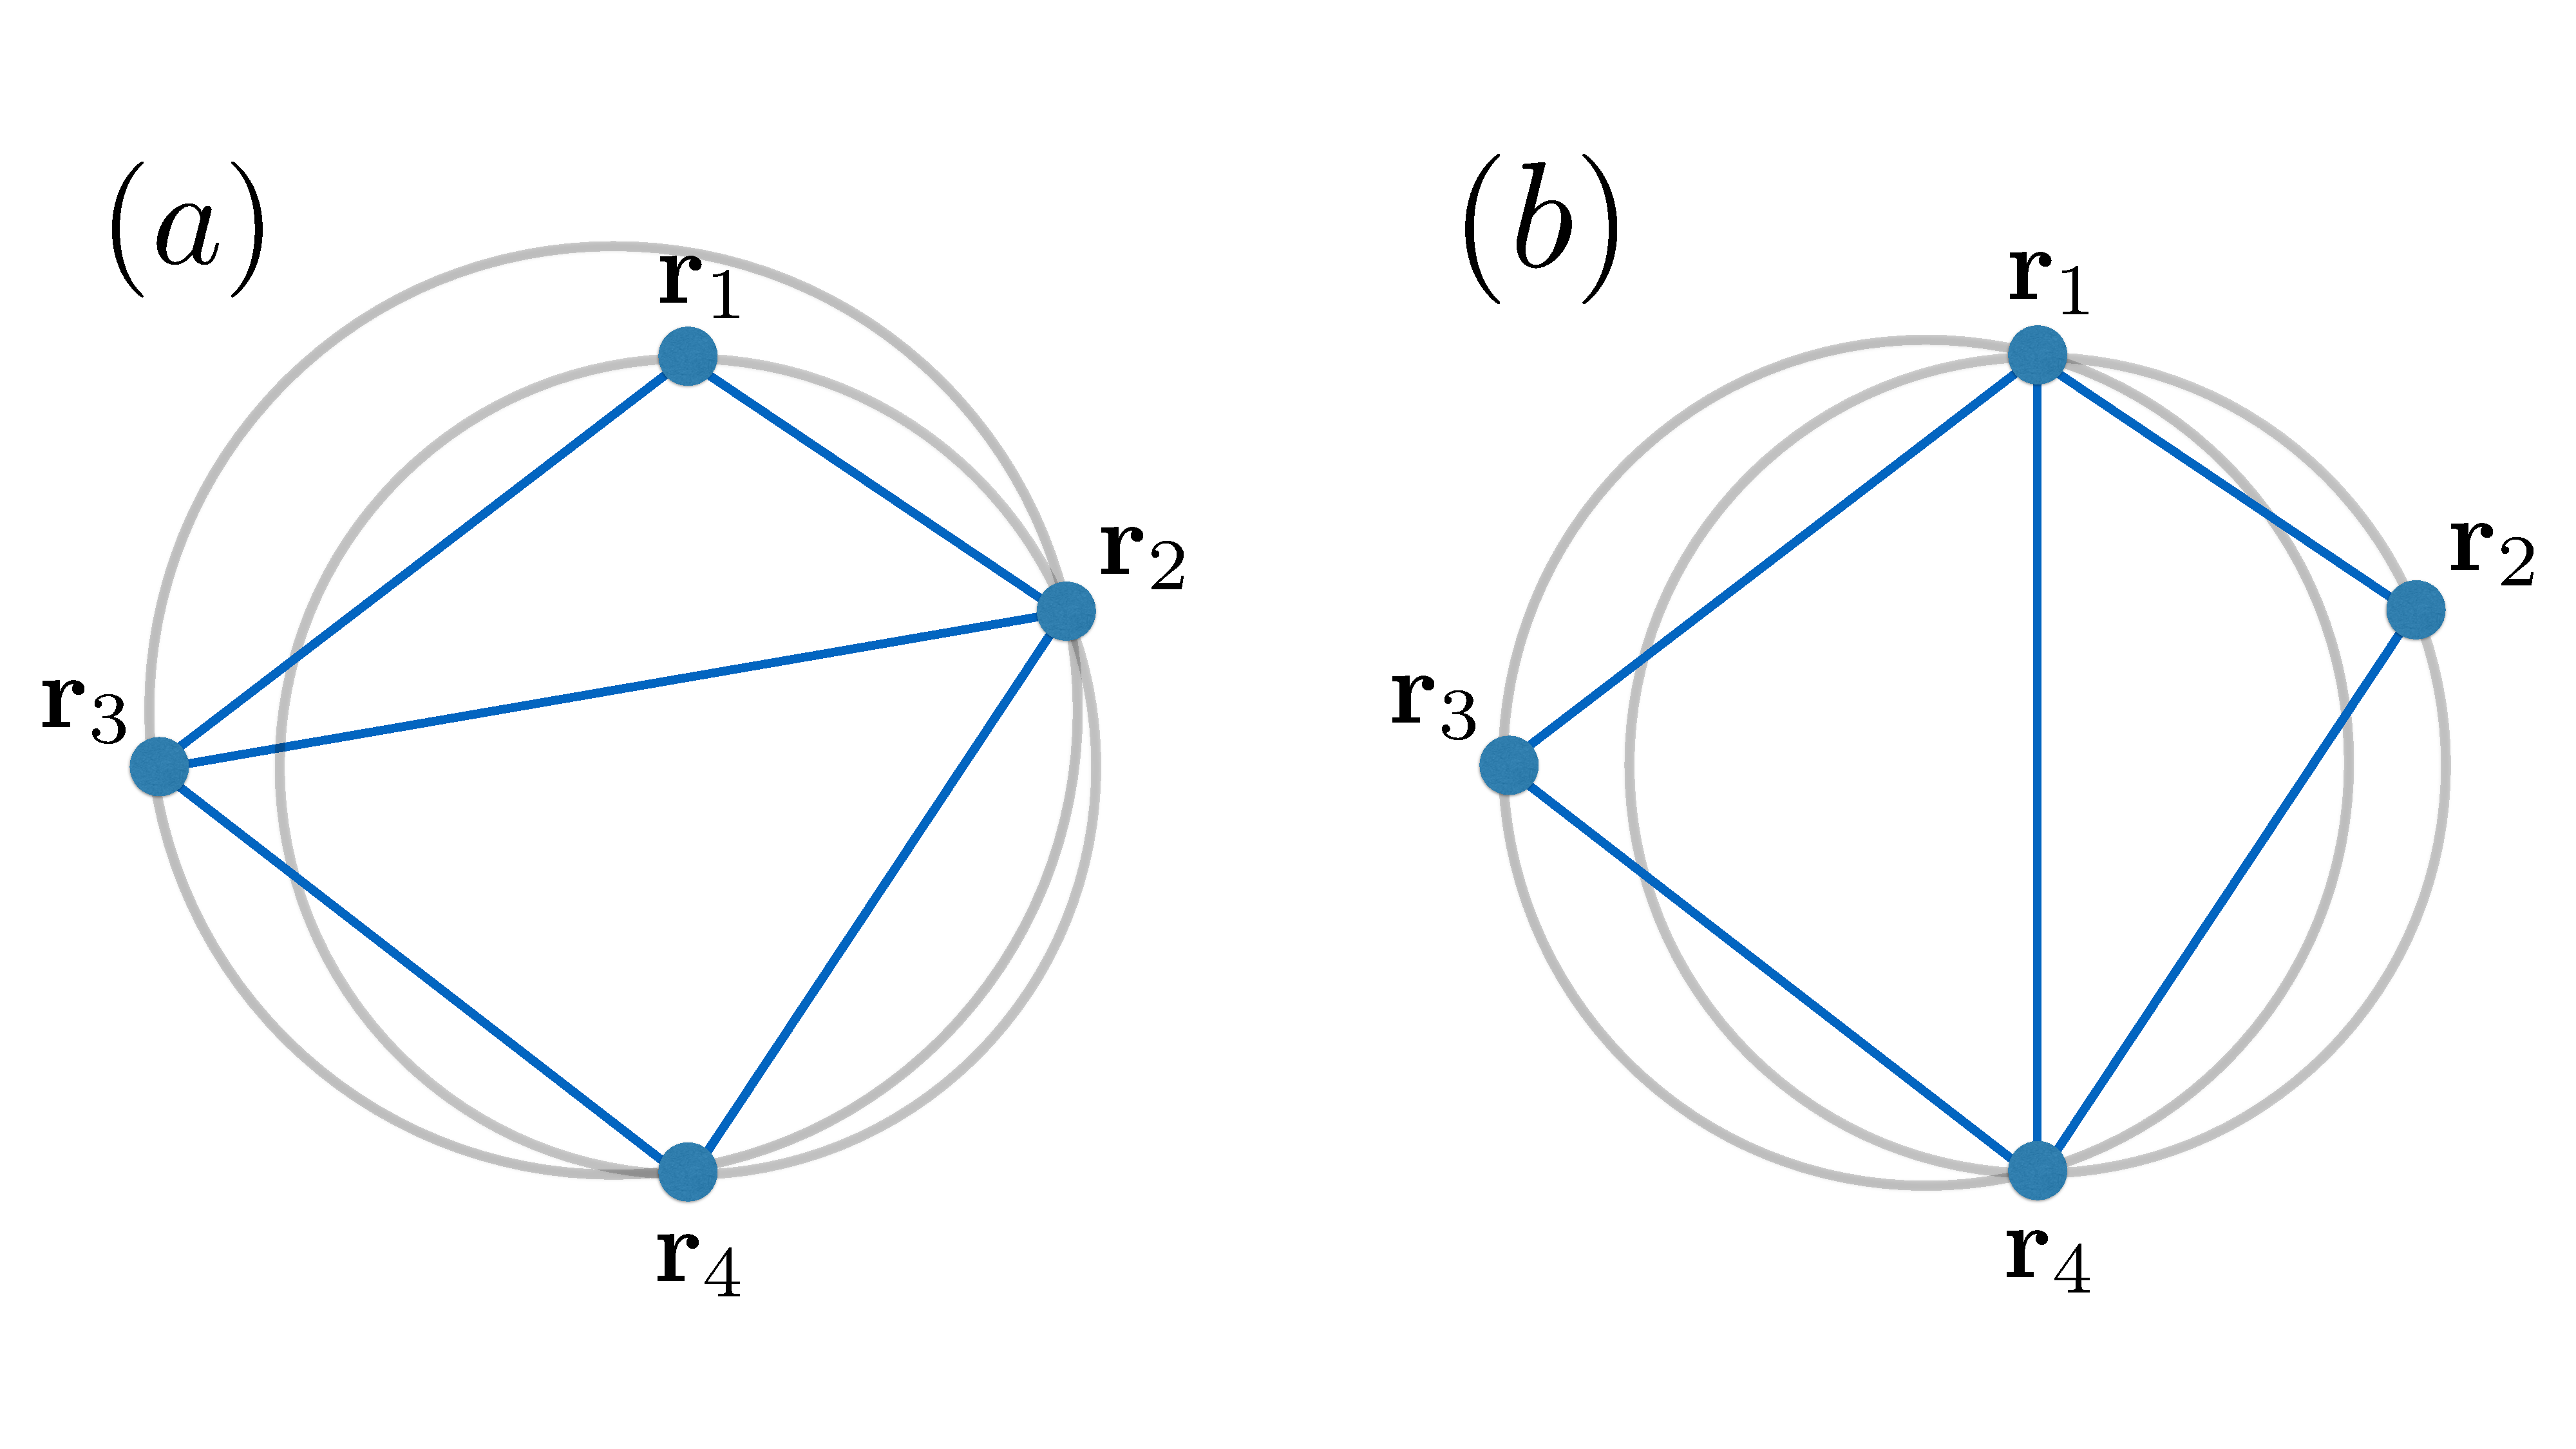
\includegraphics[width=0.85\textwidth]{Images/ch6_phasegineer/imgs/delaun}
    \caption{Non-Delaunay (a) and Delaunay (b) triangulation of 4 Euclidian points.}\label{fig:delaun}
\end{figure}
This concept is more easily explained visually. Fig.~\ref{fig:delaun} shows two different triangulations of four points;  \ref{fig:delaun}(a) is a non-Delaunay triangulation, as the point $\mathbf{r}_1$ falls within the circumcircle of the other points. However, by simply flipping the central edge from $(\mathbf{r}_2, \mathbf{r}_3)$ to $(\mathbf{r}_1, \mathbf{r}_4)$ we can see that we now have a legal Delaunay triangulation with $(b)$. No point falls within the circumcircle of the other points, and the minimum angle formed is maximised relative to configuation $(a)$. Following directly from this one can see that Delaunay triangulation can be used to connected the closest vertices in a network. A nice side-effect of Delaunay triangulation is that one can examine the appearance of vertices with a different number of edge connections to the norm. This can be a useful means to locate defects in a crystal lattice, and I will make use of this during later discussions.

An alternative representation, using the dual of the Delaunay triangulation, is that of the Voronoi diagram. The characteristic of these diagrams is that they are composed of cells each encompassing an individual vertex, within which all area is closer to that particular vertex than any other. This can be generated from the Delaunay triangulation and vice-versa. Taking the centres of the circumcircles decribing the Delaunay triangulations, and connecting these forms the boundaries of the voronoi cells. A simple generation method can be seen as creating and expanding the radius of circles (or n-spheres in n-dimensions) centred on each vertex. Where circles intersect with one another defines the boundary of each individual cell. An example of a Voronoi diagram compared with a Delaunay triangulation is given by Fig.~\ref{fig:voronoi}.
\begin{figure}\centering
    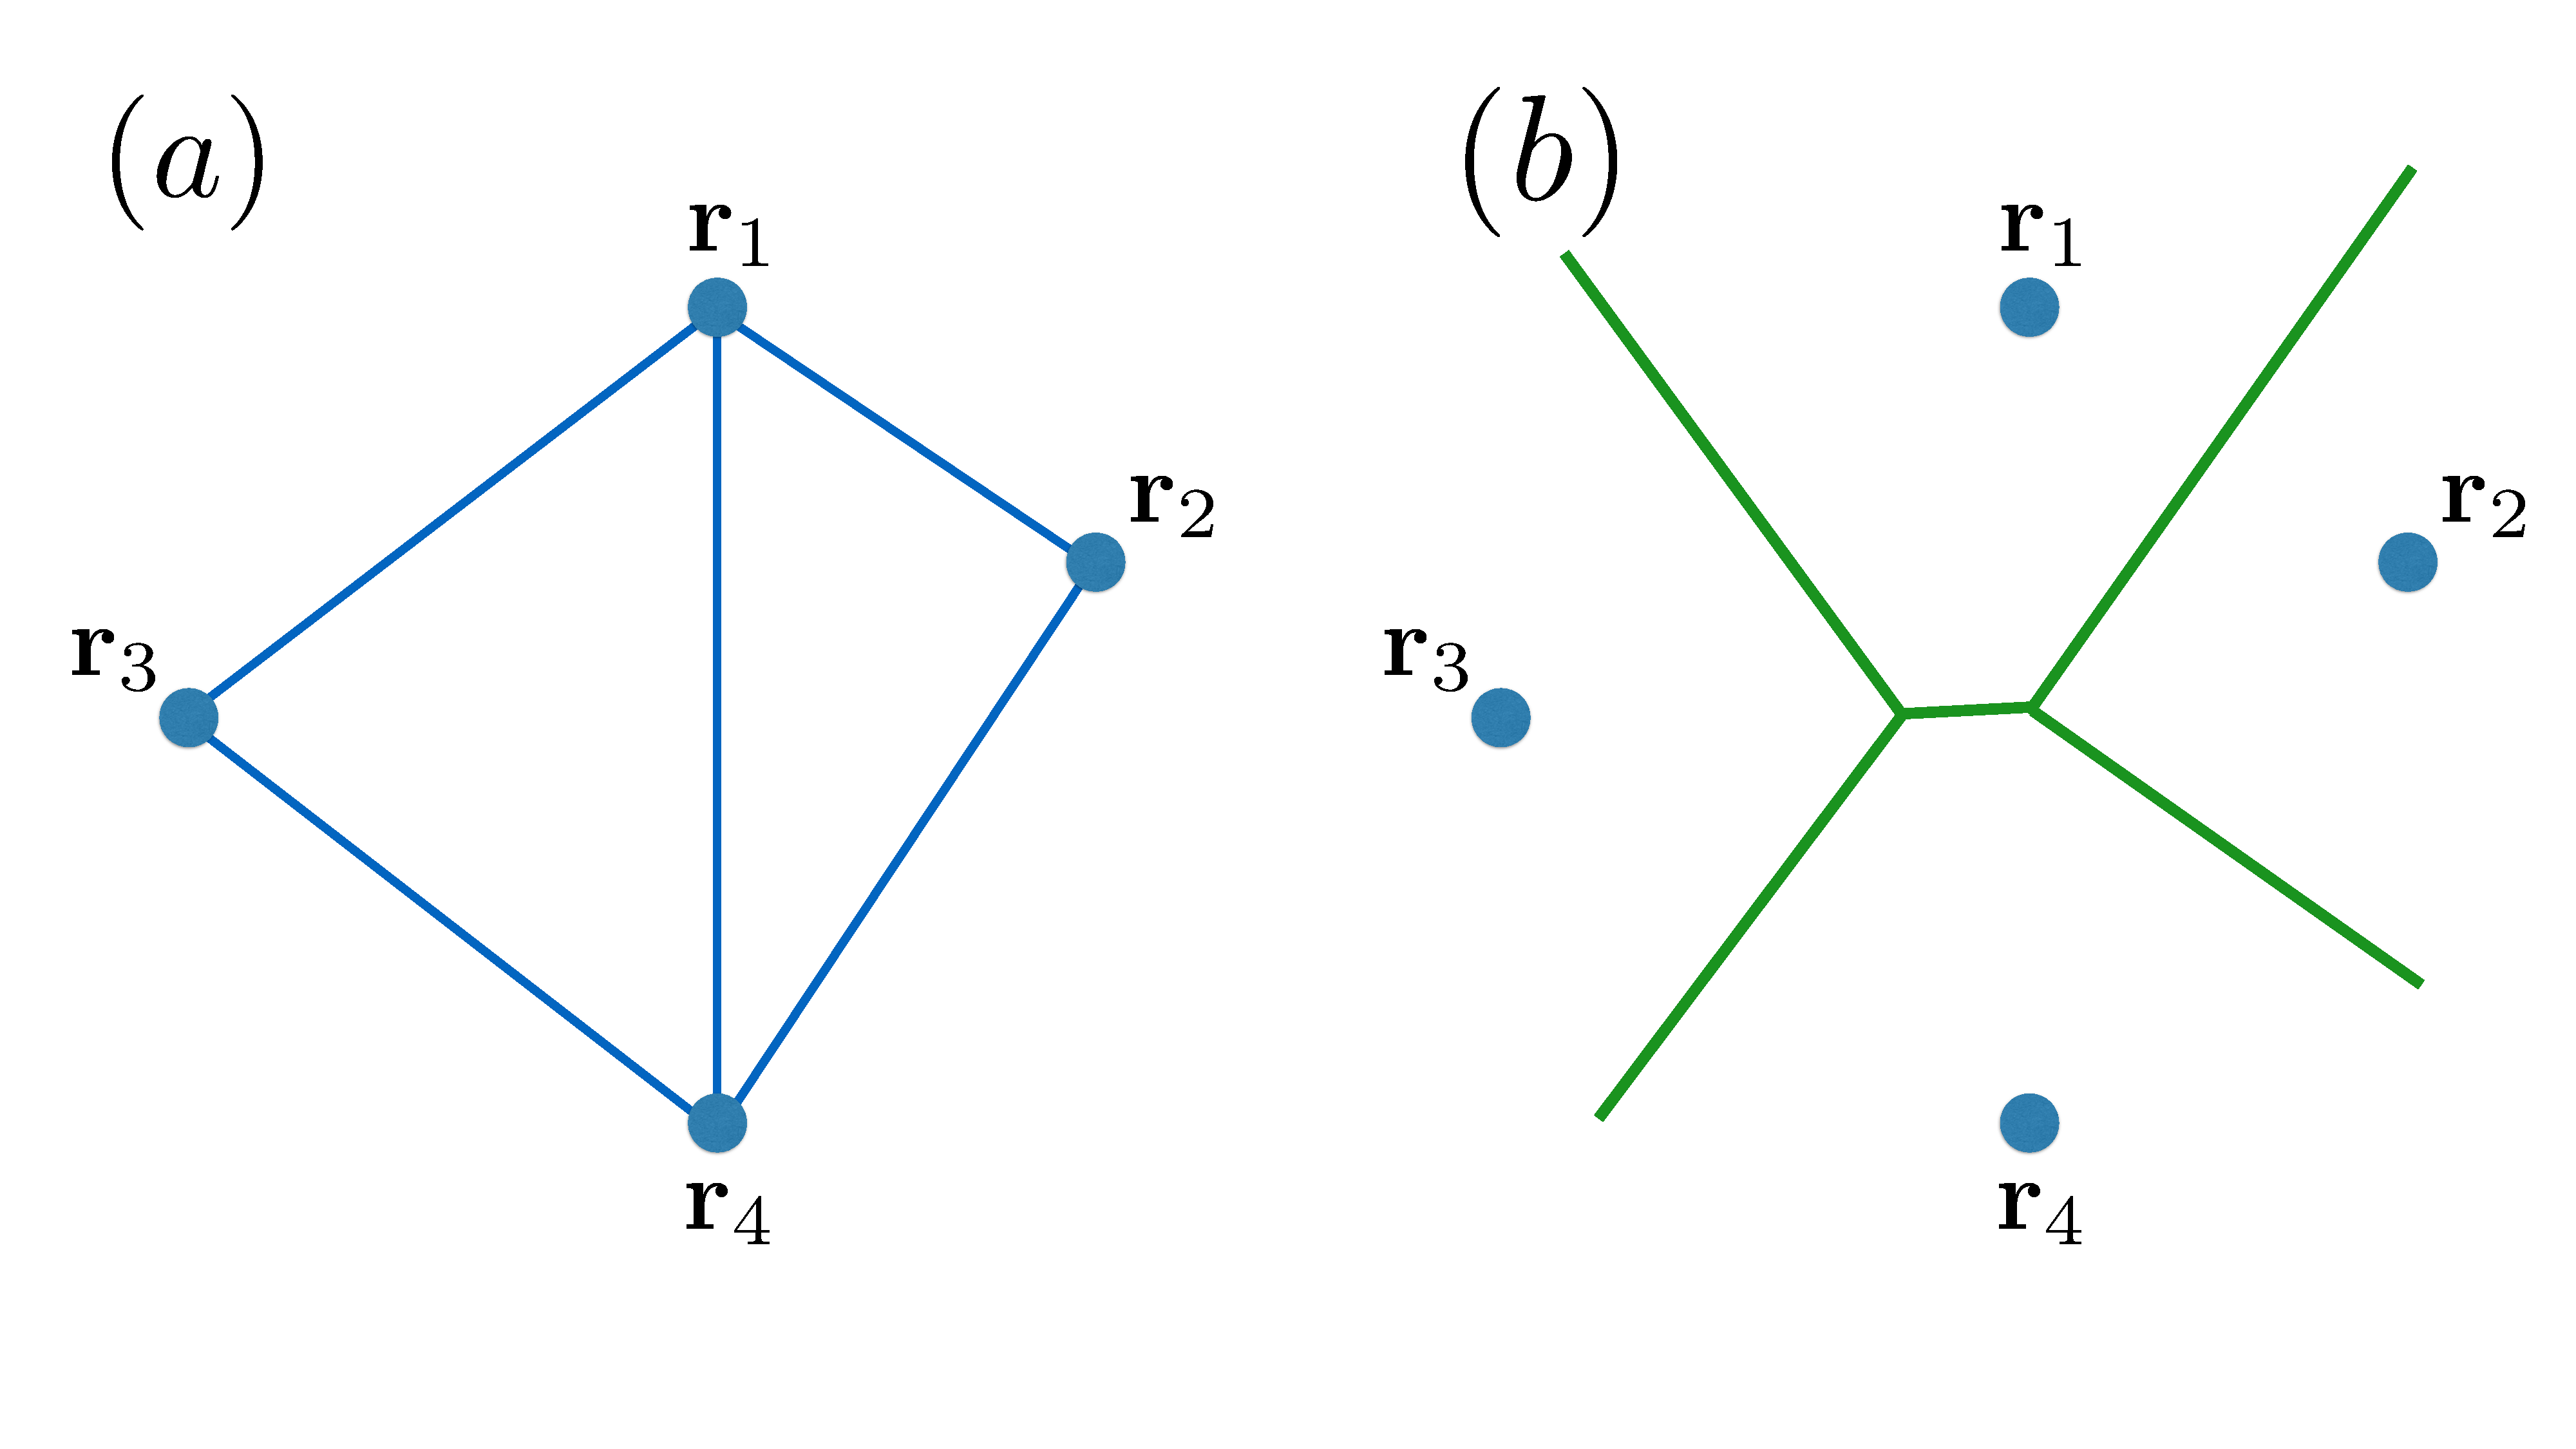
\includegraphics[width=0.85\textwidth]{Images/ch6_phasegineer/imgs/voronoi}
    \caption{Comparison of Delaunay triangulation $(a)$ with a Voronoi diamgram $(b)$. These graphs are duals, and if given one, can be used to generate the other.}\label{fig:voronoi}
\end{figure}
The area of each cell can be used as a metric of the strength of the bonding in a many-body system, but also we may represent quantities local to each region in a system by the colourscale of each cell.
